\documentclass[preprint,linenumbers, longauthor]{aastex631}
\usepackage{graphicx}
\usepackage{appendix}
\usepackage{listings} 
\usepackage{xcolor}
\begin{document}

\title{The New Age of Big Data In Astronomy: A Review of on the SKA \& Rubin/LSST}
\author{Mathew Icho}
\affiliation{The University of Illinois at Urbana-Champaign}

\begin{abstract}
I'm making my abstract my to do list for now

\textbf{NOTE: I fixed the things you told me to fix, I added a new figure to sdss section, I added lsst section}


\textbf{1. Fix the SDSS part based on provided notes, also make real-time processing section}

\textbf{2. Find a paper or part of it that describes how SDSS stores the data. I don't think I've dont that sufficiently}

\textbf{3. Do the LSST part}

\textbf{4. Do the Results section, look at data collected. I plan on coding A LOT for this section}

\textbf{5. Redo the Du Pont section, it's outdated}

\end{abstract}

\tableofcontents

\section{Introduction}
%Start with kind of a summarized overview with the paper
%Then go to history of data being handled in Astronomy
%Then go talk about Moore's law%Then talk about main idea of this paper, say how its gonna be structured
The concept of data has long been central throughout the history of astronomy. Data allows scientists to discover natural laws in the universe, have control over events, and make reliable predictions. It has played a critical role in other time-sensitive fields such as medicine and engineering, where accurate data is essential for decision-making and design. 
Although the nature of data varies fundamentally across different fields, one trend has remained consistent: the continual evolution of data science. As explained in The Fourth Paradigm \citep{heyFourthParadigmDataIntensive2009}, this evolution can be characterized through four successive paradigms. 
In the following sections, I describe the progression of data acquisition across these paradigms and illustrate each using examples from astronomy. I will then explain how SKA and LSST fit into this trajectory and exemplify the emerging era of data-intensive discovery.
\subsection{The Paradigms of Data Science}
The first and most primitive paradigm, as described by \cite{heyFourthParadigmDataIntensive2009}, is empirical evidence. 
Empirical evidence refers to data collected through traditional means, such as direct observation or experimentation. 
The primary purpose of empirical evidence is to identify patterns that allow scientists to develop a fundamental understanding of the natural world. 
Throughout much of human history, empirical evidence has dominated knowledge generation. 
An example of the first paradigm in astronomy is the career of Tycho Brahe, a Danish astronomer. Throughout his career in the 16th century, Brahe collected and cataloged data on the position of astronomical bodies using naked-eye observations. 
However, empirical evidence can be compromised by human error, the precision of the instruments, and, most importantly, the relatively slow pace of data acquisition compared to subsequent paradigms.

The second paradigm is analytical evidence. Analytical evidence is obtained by constructing mathematical formulas and theoretical frameworks based on empirical data \cite{heyFourthParadigmDataIntensive2009}. 
Unlike the empirical evidence, which merely demonstrates that phenomena occur, the second paradigm seeks to explain why they occur. 
An example of the second paradigm in astronomy is the work of Johannes Kepler, who used Brahe's empirical observations to derive the laws of planetary motion \citep{heyFourthParadigmDataIntensive2009}. 
By transforming raw observational data into mathematical laws, Kepler exemplified how analytical evidence advances scientific understanding beyond description to explanation.

The third paradigm is simulation evidence \cite{heyFourthParadigmDataIntensive2009}, a relatively recent development. Simulation models natural phenomena that are too complex to model analytically or compute by hand. 
It allows interpolation and extrapolation of data using computational techniques grounded in known physical laws. 
For example, in astronomy, N-body simulations are used to study the complex dynamical evolution of planetary systems and galaxies. 

The fourth and most recent paradigm is data-intensive science \cite{heyFourthParadigmDataIntensive2009}. 
This paradigm is characterized by the unprecedented scale, velocity, and complexity of data acquisition, driven in part by exponential advances in computational power and detector technologies, often associated with Moore's law \cite{heyFourthParadigmDataIntensive2009}. 
Unlike earlier paradigms, which focused on observation, theory, or simulation, data-intensive science emphasizes the ability to manage, analyze, and interpret vast datasets that exceed the capacity of traditional methods. 
While this exponential growth in data has enabled transformative discoveries, it also introduces significant challenges related to storage, processing, and accessibility. 

\subsection{The Rise of Big Data in Astronomy}
Astronomy has become data intensive. Modern observatories may now generate petabyte-scale data that need new strategies for data management and analysis \cite{heyFourthParadigmDataIntensive2009}. 
The fourth paradigm enables discoveries from interpreting massive data sets. 
However, these advances also expose alarming issues, including bottlenecks in the data pipeline, storage challenges, increased skills needed to handle the data, and open access concerns. 
The field of astronomy is both a beneficiary and a victim of this data-intensive transition. 

As mentioned above, the exponential growth of data acquisition can be attributed to Moore's law \cite{heyFourthParadigmDataIntensive2009}.  
Moore's law predicts that integrated circuit chip density doubles approximately each year at a fixed price point \cite{mooreCrammingMoreComponents2006}.
\cite{mooreCrammingMoreComponents2006} questioned whether technical development would sustain the growth.

Moore's law can be seen in many data-intensive fields, including astronomy.
It explains both the recent development of big data in astronomy, and predicts future challenges.

This paper therefore seeks to review the rise of big data in astronomy and the technical and scientific issues surrounding it by examining four case studies: MeerKAT \footnote{https://www.skao.int/en}, The Sloan Digital Sky Survey (SDSS) \footnote{https://www.sdss.org/}, The Legacy Survey of Space and Time (LSST) \footnote{https://www.lsst.org/}, and The Square Kilometre Array (SKA) \footnote{https://www.skao.int/en}. 
These facilities represent the scope of contemporary astronomical data, the methods of its acquisition, their relative successes, the ongoing challenges, and the solutions currently in use.

\subsection{An Overview of The Four Surveys}
The SDSS is vital to this paper, as it is one of the earliest large-scale optical surveys that marks the start of the fourth paradigm. 
The SDSS is a precursor to LSST. The SDSS
consists of three main telescopes.

The first of the three is The Sloan Foundation 2.5m Telescope. 
The Telescope is stationed at the Apache Point Observatory in New Mexico, where it observes the sky in the northern hemisphere. 
It is able to observe a 3$^\circ$ field of view by use of two corrector lenses \citep{gunn25TelescopeSloan2006}.

The SDSS also uses the Irénée du Pont telescope at Las Campanas Observatory \footnote{https://www.lco.cl/irenee-du-pont-telescope/}. This telescope is stationed in Chile, where it observes the southern hemisphere instead. 
Similar to the foundational telescope at Apache Point, this telescope has a 2.1$^\circ$ field of view but only uses one corrector lens \cite{bowenOpticalDesign40in1973}.

The third telescope is the NMSU 1-meter Telescope \footnote{https://newapo.apo.nmsu.edu/}. The NMSU telescope is stationed at the Apache Point Observatory alongside the foundational telescope. 
The NMSU telescope is designed to observe bright stars that are too bright for the aforementioned two telescopes to observe \citep{majewskiApachePointObservatory2017}. 

the SDSS is made up of multiple subsurveys. The eBoss survey \footnote{https://www.sdss4.org/surveys/eboss/}, a continuation of BOSS, uses spectrographs to observe light in a wavelength range of 3600-10,400~\AA \space \citep{dawsonSDSSIVEXTENDEDBARYON2016}.
An additional subsurvey is APOGEE-2, a continuation of APOGEE. It uses spectrographs similar to eBOSS, but APOGEE-2 collected near-infrared spectra \citep{majewskiApachePointObservatory2017}. 
MaNGA \footnote{https://www.sdss4.org/surveys/manga/} is a subsurvey that collects integral field unit spectra of 10,000 nearby galaxies \citep{bundyOVERVIEWSDSSIVMaNGA2014}.
MARVELS \footnote{https://www.sdss4.org/surveys/marvels/} is another SDSS subsurvey, it was built specifically to obtain radial velocity measurements of stars with high-precision in hopes of finding exoplanets \citep{bundyOVERVIEWSDSSIVMaNGA2014a}.


The MeerKAT \footnote{https://www.sarao.ac.za/science/meerkat/} is an important precursor telescope to the SKA \citep{jonasMeerKATRadioTelescope2018}
MeerKAT became fully operational in 2018 in the Northern Cape Province of South Africa.
MeerKAT comprises 64 antennas distributed over a radius of approximately 600 miles \cite{goedhartMeerKATSpecifications2025}. These antennas operate across frequency bands ranging from 350 MHz to 3500 MHz \citep{goedhartMeerKATSpecifications2025}.

MeerKAT has conducted and continues to conduct ten major survey projects \citep{jonasMeerKATRadioTelescope2018}. For conciseness, this discussion will focus on five of these surveys.
One is the LADUMA \footnote{https://science.uct.ac.za/laduma} survey.
The objective of the LADUMA survey is to use HI obversations to research galaxy evolution over approximately 9.8 billion years \citep{blythLADUMALookingDistant2018}. 
LADUMA has used MeerKAT's Phase 1 receivers, which cover 0.9-1.75 GHz. It later transitioned to longer observations in Phase 4, which cover the 0.58-2.5 GHz band \citep{blythLADUMALookingDistant2018}.
Although the LADUMA survey is still ongoing, a portion of the data has already been released and will be discussed in the Methods section.

The MeerKAT absorbtion line survey \footnote{https://mals.iucaa.in/} (MALS) is a survey of HI and OH absorbers at a redshift of $z < 0.4$ and $z < 0.7$. 
HI is a descriptive tracer of the cold neutral medium in a galaxy \citep{guptaBlindOHAbsorption2021}. 
The cold neutral medium contains the physical conditions of the interstellar medium of each galaxy. This, in turn, allows scientists to estimate star formation rate in the galaxy \citep{guptaBlindOHAbsorption2021}.

Another survey, ThunderKAT \footnote{https://www.physics.ox.ac.uk/research/group/meerkat}, aims to find, identify and understand high-energy radio transients, usually grouped with observations at similar wavelengths.
Examples include supernovae, microquasars, and similar events \citep{woudtThunderKATMeerKATLarge2018}.

Another notable MeerKAT survey is MHONGOOSE \footnote{https://mhongoose.astron.nl/}. This survey aims to catalogue the properties of HI gas using 30 nearby star-forming spiral and dwarf galaxies. 
MHONGOOSE is remarkable for its higher sensitivity compared to previous surveys such as HALOGAS \footnote{https://www.astron.nl/halogas/} and THINGS \footnote{https://www2.mpia-hd.mpg.de/THINGS/Overview.html} \citep{deblokMHONGOOSEMeerKATNearby2024}. 
This sensitivity is crucial for investigating how low-column-density gas influences the cosmic web and galactic accretion processes \citep{deblokMHONGOOSEMeerKATNearby2024}.

The final MeerKAT survey considered here is MIGHTEE \footnote{https://www.mighteesurvey.org/home}. MIGHTEE spans 900-1670 MHz, achieving a resolution of approximately 6 arcseconds. MIGHTEE seeks to study the evolution of active galatic nuclei, neutral hydrogen, and the properties of cosmic magnetic fields \citep{MIGHTEESurvey}.

\begin{figure}[h!]
  \centering
  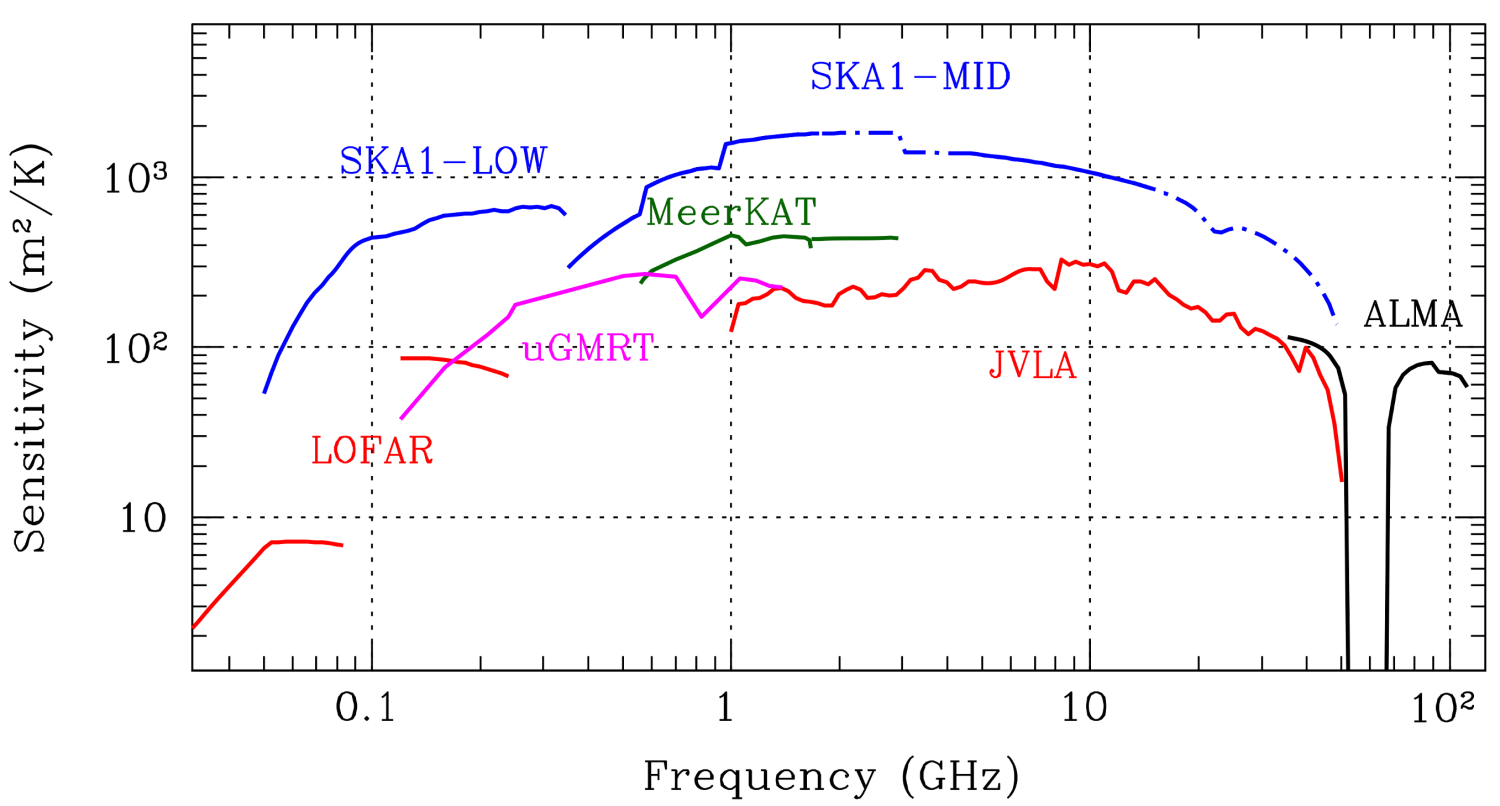
\includegraphics[width=0.8\textwidth]{SKA_Graph.png}
  \caption{Figure from the SKA Official website, demonstrating the sensitivity compared to similar observatories}
  \label{fig:SKA_Graph}
\end{figure}

The SKA has built on technical and scientific achievements paved by MeerKAT and other radio interferometers.
The SKA covers an area of approximately 131,205 antennas \citep{SKATelescopeSpecifications}. The SKA represents the start of a new frontier for big data in astronomy.
As an interferometer it uses aperture synthesis, which allows for the signals from antennas to be phased, this allows to reduce noise \citep{dewdneySquareKilometreArray2009}. The SKA will be discussed in further detail in the Methods section. 

Alongside the SKA is its optical big data counterpart, the LSST.
As noted above, the LSST is a successor to the SDSS. Rubin/LSST, however, has much more sophisticated goals. The LSST plans to address four key scientific issues:Investigating dark energy and dark matter, cataloguing the solar system, collecting data for sky surveys, and mapping the Milky Way.
To achieve this, the LSST uses a 3.2-gigapixel camera with a sampling of 9.6 deg$^2$ field of view \citep{ivezicLSSTScienceDrivers2019}. These cameras are equipped with highly resistant sensors reinforced with silicon \citep{ivezicLSSTScienceDrivers2019}. Rubin/LSST has an unprecented data rate for an optical telescope.

The SDSS, MeerKAT, SKA, and LSST generate unprecedented data rates and allow the experimentation of complex astrophysical events and phenomena.
In the following Methods section, I describe how the data are collected, processed, analyzed, and stored. I then compare SDSS and MeerKAT to their larger successor telescopes, Rubin/LSST and SKA and consider the evolution of data challenges.

\section{Methods}

%Methods:
%○ Approach to collecting Data
%● Talk about how the LSST and SKA are collecting data
%○ The nature of their data, ie the scope, type, etc
%■ LSST is optical imaging
%■ SKA is radio interferometry
%○ How they’re storing/archiving the data.
%○ How they’re generally processing their data
%○ Transparency of their respective Data pipeline
%○ Real time processing techniques (NOTE: NOT THE SAME AS THE METHODS
%DATA PROCESSING, THIS ONE IS FOR REAL TIME PROCESSING)
    %■ Show new techniques being developed to combat issues such as
    %optimization and time important issues

%LSST FIRST??
\subsection{The Optical Big Data Pipeline}

This section carefully examines how each of the optical focused surveys collects and processes its data. 
It begins by describing the nature, scope, and type of the data. 
Next, it discusses how each survey collecs and archives its data, followed by an explanation of their general data processing methods. 
Finally, it considers the use of real-time data processing. 
By comparing these surveys, this study highlights the rapid growth of big data in astronomy, a trend that has created challenges for data storage, processing, and analysis. 
These challenges will be discussed further in the discussion section.

The first survey examined is the Sloan Digital Sky Survey (SDSS). The SDSS I plan on splitting  the SDSS into its three main components, the 2.5 m Telescope, the Irénée du Pont Telescope, and the NMSU 1-meter telescope.
As discussed previously, I will explain how each telescope collects data, then I will explain how the SDSS processes the data both generally and in real-time. 
Lastly, I will talk about the open data policy the SDSS has employed.


\subsubsection{The Sloan Digital Sky Survey (SDSS)}
\paragraph{Data Collection and Storage} 
Although the SDSS is a complex survey, it can be divided into several major components, each of which contributes to the collection of astrophysical data.
The 2.5-meter telescope plays a central role in the operations of the SDSS. It was designed to conduct precise optical observations of the sky over many years. 


\textbf{(1) The SDSS 2.5 m Telescope:}  
According to Gunn et al. (2006), the SDSS camera contains “30 2048 x 2048 Scientific Imaging Technologies Charge-Coupled Devices (CCDs) and 24 2048 x 400 CCDs” \cite{gunn25TelescopeSloan2006}. 
A CCD is a detector that converts incoming light into an electronic signal. 
When photons strike the CCD, they generate electrons through the photoelectric effect. 
Using applied voltages, the resulting charge is measured based on the number of electrons produced. 
That measurement is then converted into a digital value and stored as a pixel, forming an image \cite{lesserSummaryChargeCoupledDevices2015}.

Another major innovation that enables the SDSS to collect data is the pair of fiber-fed double spectrographs, which record imaging data across wavelengths from 3800 to 9200~\AA\ and at field angles between 0 and 90$^{\circ}$ \cite{gunn25TelescopeSloan2006}. 
present measurements of the optical performance of these instruments, which are summarized in Figure~\ref{fig:SDSS_Table}.

\begin{figure}[h!]
  \centering
  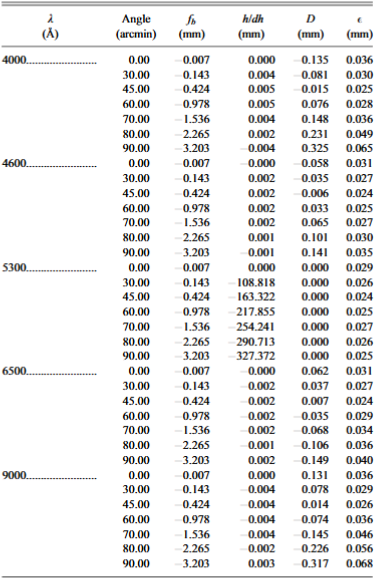
\includegraphics[width=0.4\textwidth]{gunn_table_5.png}
  \caption{Figure 5 from Gunn et al. (2006), showing results of the SDSS spectrographs given Wavelength and Angle.}
  \label{fig:SDSS_Table}
\end{figure}

In Figure~5, $\lambda$ represents the wavelength of light, and “Angle” refers to the field angle. 
$f_b$ is the best-focus distance, which is the position that provides the sharpest image. 
$h/dh$ represents the lateral color, and $D$ indicates the longitudinal difference from the best focus. 
Finally, $\epsilon$ is the root mean square (rms) image diameter. 
Among these parameters, the lateral color and longitudinal difference are the most important for image quality because smaller values indicate sharper images. 
Based on the data from \cite{gunn25TelescopeSloan2006}, both of these quantities remain close to zero for most wavelengths and field angles, except between roughly 5300 and 6500~\AA, which demonstrates the high optical accuracy of the SDSS spectrographs.

The combination of these two innovations alongside others help the 2.5 m telescope collect data at a rate of about 20Gb/hr \cite{luptonSDSSImagingPipelines2007}.

\textbf{(2) The Irénée du Pont Telescope:}  
Unlike the 2.5 m telescope, the Du Pont Telescope does not rely on CCDs to collect data. According to Bowen's 1973 paper, the telescope is described as a modified Ritchey-Chrétien design with Gascoigne correctors \cite{bowenOpticalDesign40in1973}.
The Du pont telescope uses a 100-inch primary mirror. Approximately 40\% of the light is reflected to the secondary mirror, obtaining only a 16\% loss of light at that stage. \cite{bowenOpticalDesign40in1973}
The combination of light from the two aforementioned mirrors are then sent to a 20 inch x 20 inch plate, where monocromatic images are formed.

The du Pont Telescope uses 18.9 inch nonvignetted plates in order to minimize vignetting \cite{bowenOpticalDesign40in1973}. Vignetting is the process where light beds through the lense of a telescope. The bending form a cone of light, which causes images to be darker near the edges and brighter in the center of the image \cite{richardsWhatVignetting2020}.
Because of the nonvignetted plates, the du Pont Telescope experiences an exceptionally low 3\% percent loss of light \cite{bowenOpticalDesign40in1973}.

Another technology the du Pont Telescope applies is a Gascoigne corrector plate. The plate helps with data collection. The Gasciogne corrector plate is able to be moved, which can help optimize the collection of light in a wanted wavelength \cite{bowenOpticalDesign40in1973}.
Given a seperation of 1000 mm from the end of the corrector plate to the focus gives an image with a minimized astigmatism for a refractive index of n = 1.47 \cite{bowenOpticalDesign40in1973}.
At a given wavelength, the change of length which minimizes astigmatism is described in Bowen's paper as

\begin{equation}
\Delta L = 590\Delta n / (n - 1) = -1250\Delta n
\end{equation}

Where $\Delta L$ is the change in seperation in millimeters and $\Delta n$ is the difference between a refractive index of 1.47 and the index wanted.

The last technology the du Pont Telescope uses is conical baffles. The reason for this is to promote shielding in the telescope \cite{bowenOpticalDesign40in1973}.
As explained in the Bowen paper, shielding is necessary in order to protect the photographic plate from light that escapes from the secondary lense due to long time exposure.
As explained in the Bowen paper, the conic baffles are "located in the space between the incoming beam as it appraoches the primary and the return beam from the secondary to the plate" \cite{bowenOpticalDesign40in1973}.
Theoretically, the conic baffles have the disatvantage of producing a diffraction pattern. However, as explained by Bowen, this should not majorly affect the images of stars \cite{bowenOpticalDesign40in1973}. 

\textbf{(3) The New Mexico State University (NMSU) Telescope:}  
The NMSU telescope takes the most technologically advanced approach to collecting data compared to the 2.5 m telescope and the du Pont Telescope.
The NMSU telescope uses a camera that has a 2048 x 2048 CCD. The camera is controled by a linux computer, which is connected by fiber optic cables \cite{holtzmanNMSU1Telescope2010}.

The data collection of the NMSU telescope is almost fully automated using C++, the only time it is not is when engineering is being done on the telescope \cite{holtzmanNMSU1Telescope2010}.
The NMSU telescope has a camera which analyzes the brightness level of the sky to see if it is dark enough to start collecting data.
When the sky becomes dark enough, the telescope initiates its program. The telescope goes through the list and observes said objects \cite{holtzmanNMSU1Telescope2010}.
Objects can, however, be observed as many times as requested. 

\paragraph{Data Processing} 
 %\textbf{NOTE: This is gonna super complex, Study this hard. Its only surface level rn } 
The SDSS processes its data through an innovative acquisition system that records and organizes observations in real time while maintaining strict quality control \cite{gunn25TelescopeSloan2006}. 
This system ensures that data are processed and stored efficiently without any loss of precision. \cite{gunn25TelescopeSloan2006}. 
The data pipeline of the SDSS can be described by two different fields of data, the imaging pipeline and the spectroscophy pipeline

 \textbf{(1) Imaging Data Pipeline:} 
  The Imaging data Pipeline itself consists of mutliple subpipelines. 
  The first subpipeline is the Astroline. The astroline uses vxWorks in order to initalize the processing sequence.
  This happens by composing star cutouts and column quartiles collected from the CCD's mentioned before \cite{luptonSDSSImagingPipelines2001}

  The second subpipline is the MT pipeline. the MT Pipeline processes the data collected from the Photometric Telescope. 
  This data is used to calculate important parameters for the 2.5 m Telescope scans, such as extinction and zero-points \cite{luptonSDSSImagingPipelines2001}.

  The third pipeline is the Serial Stamp Collecing (SSC) Pipeline. the SSC reorganizes the star cutouts collected from previous pipelines.
  The SSC does this in order to prepare data for the upcoming pipelines \cite{luptonSDSSImagingPipelines2001}.

  Next is the Astrometric Pipeline. The Astrometric pipeline processes the average location of stars using the data collected from the astroline and SSC pipelines. 
  It then converts the pixel data from the images into celestial coordinates ($\alpha, \delta$) \cite{luptonSDSSImagingPipelines2001}.

  After that is the Postage Stamp Pipeline (PSP). 
  The PSP estimates the quality of the data collected by calculating factors such as the flat field vectors, bias drift, and sky levels \cite{luptonSDSSImagingPipelines2001}.

  After all that is done, the data is fed into the Frames Pipeline. The Frames pipeline does a majority of the work, processing the data from all the previous pipelines and producing the complete datasets of images.
  It does this by correcting the frames based on the data before and cataloging the images \cite{luptonSDSSImagingPipelines2001}.

  Lastly, the processed data is then ran through the Calibration pipeline. The Calibration pipeline takes data from the MT and Frames pipeline. The Calibration pipeline converts the counts into more measurable quantities such as flux \cite{luptonSDSSImagingPipelines2001}.

The SDSS imaging pipeline is composed of multiple connected pipelines that operate collaboratively to transform raw imaging data into structured datasets from which measurable physical quantities such as flux can be derived.

\paragraph{Real-Time Processing} 

\subsubsection{The Rubin/Large Synoptic Survey Telescope (LSST)}
\paragraph{Data Collection and Storage}
Despite the recent times in creation. The SDSS collected around 16 TB of data over a decade in their data release 7 \citep{juricLSSTDataManagement2017}. Yet the LSST is expected to collect 20 TB of data per night \citep{nsf-doeverac.rubinobservatoryPSTN019LSSTScience2025}.

The LSST pipeline is written with around 750000 in Python in order to use relevant libraries such as SciPy and AstroPy \citep{nsf-doeverac.rubinobservatoryPSTN019LSSTScience2025}.
The pipeline is also written with around 220000 lines in C++ in order to ensure efficient performance \citep{nsf-doeverac.rubinobservatoryPSTN019LSSTScience2025}.
In order to combine these two languages, pybind11 allows for the transition from Python to C++, and ndarray objects are able to be converted from C++ arrays \citep{nsf-doeverac.rubinobservatoryPSTN019LSSTScience2025}.

The python enviroment of the LSST pipeline uses a package named \texttt{rubin-env}. This package gives the user all the code needed to run LSST's data. 
In order to execute the code, the pipeline consists multiple packages that each serve their own purpose. 
The LSST has defined a class labled \texttt{Task}, which is used to define algorithms \citep{nsf-doeverac.rubinobservatoryPSTN019LSSTScience2025}.

One instance of a task is the \texttt{PipelineTask}, which serves to organize subtasks. These subtasks each have their own purpose \citep{nsf-doeverac.rubinobservatoryPSTN019LSSTScience2025}. 
The most important subtask, labeled \texttt{daf\_butler}, handles the data storage. This subtask is titled by the LSST as The Data Butler. The Butler serves as a database to store collected data. It stores objects with data IDs similar to SQL, with headers that hold useful information \citep{nsf-doeverac.rubinobservatoryPSTN019LSSTScience2025}.
An example of this would be a data coordinate labeled \texttt{instrument}="LSSTCam", \texttt{exposure}=299792458, \texttt{detector}=42, \texttt{band}=z, \texttt{day\_obs}=20251011.



\paragraph{Data Processing} 
This task first Before the LSST analyzes data, it removes noise. An example of noise would be \textbf{LOOK AT 5.1 TO FINISH THIS}.

There are multiple tasks which define how the LSST processed data to find objects. These are all defined in the \texttt{meas\_algorithms} package \citep{nsf-doeverac.rubinobservatoryPSTN019LSSTScience2025}.
The task that first handles processing the catalogued images is the \texttt{SourceDetectionTask} \citep{nsf-doeverac.rubinobservatoryPSTN019LSSTScience2025}. 
This task uses Gaussian smoothing in the point spread function. It then convolves the collected image with the point spread function in order to suppress potential noise \citep{nsf-doeverac.rubinobservatoryPSTN019LSSTScience2025}.

Another task that the LSST uses to process data is \texttt{MaskStreaksTask} \citep{nsf-doeverac.rubinobservatoryPSTN019LSSTScience2025}. The task serves to mask pixels from streaks from other satellites. It identifies streaks using a Canny Filter and the Kernel-Based Hough Transform \textbf{Note: Fix this citation } \citep{nsf-doeverac.rubinobservatoryPSTN019LSSTScience2025}.
This task is combined with the deblending of collected images allows for the LSST to accurately identify objects.

\paragraph{Real-Time Processing}

\paragraph{Open Source Policies and Transparency}


\subsection{The Radio Big Data Pipeline}
\subsubsection{The MeerKAT}

\subsubsection{The Square Kilometre Array (SKA)}

\section{Results}
\subsection{}

\section{Discussion}
\subsection{Open Source Policies and Transparency}

\subsubsection{The SDSS Policy}

The SDSS collaboration states on its official SDSS-IV website \footnote{\url{https://www.sdss4.org/dr17/software/}} that all of its software be open source using the open source liscence BSD 3-Clause.
However, the SDSS outlines practices for users who plan to use the SDSS software must abide by. One of the most important ones is the proper citation of software and websites that were used. 
The SDSS4 emphasizes the importance of citing properly as it serves to acknowledge the hard work of the teams behind said projects.

\begin{figure}[h!]
  \centering
  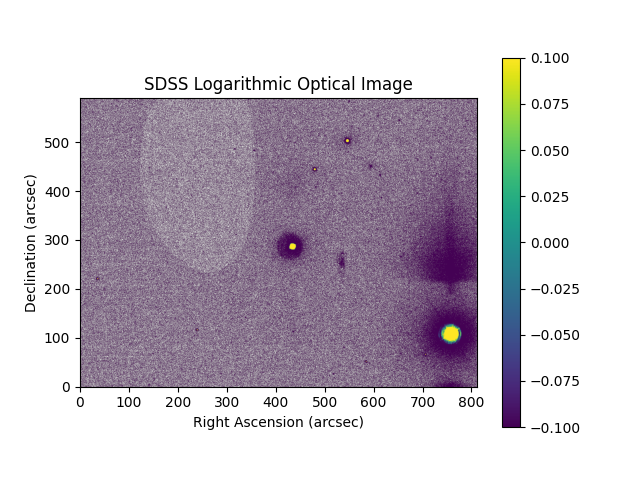
\includegraphics[width=0.5\textwidth]{SDSS_Optical_Image.png}
  \caption{A spectrographical image obtained using data collected from SDSS}
  \label{fig:SDSS_Optical_Image}
\end{figure}

The SDSS also has implemented Digital Object Identifiers, commonly known as DOIs, into all software code. DOIs allow for software and data to be easily identified, which is important for ownership.
The SDSS team also promotes transparency in coding by implementing Git and SVN in order to maintain a record of the development of the software. This not only makes the development transparent, but also helps users see the evolution of the software.

Overall, the SDSS has demonstrated a strong commitment to making their data and software open source and transparent. This in turn helps the development of science, by ensuring that knowledge is accessible to those without sufficient financial resources. 

\subsubsection{The LSST Policy}
Similar to the SDSS, the LSST has declared a commitment to having their software open source and their pipeline transparent.

\subsubsection{The MeerKAT Policy}

\subsubsection{The SKA Policy}

\lstset{
    basicstyle=\ttfamily\small,
    backgroundcolor=\color{gray!10},
    frame=single,
    breaklines=true,
    keywordstyle=\color{blue},
    commentstyle=\color{gray!70}\itshape,
    stringstyle=\color{orange},
    numbers=left,
    numberstyle=\tiny,
    stepnumber=1,
    numbersep=8pt,
    captionpos=b
}


\begin{appendices}

\section{Python Code for SDSS Data Retrieval (Figure 3)}
\label{Appendix}
\begin{lstlisting}[language=Python]
#Import relevant libraries/functions
from astroquery.sdss import SDSS
from astropy import coordinates as coords
import astropy.units as u
import matplotlib.pyplot as plt
import numpy as np

#Initalize Right Ascension and Declination
ra = 20
dec = -10

#Convert ra and dec into a SkyCoord Object
coord = coords.SkyCoord(ra, dec, unit='deg', frame = 'icrs')

#Query the SDSS System to find object given coordinates in a radius of 0.01 degrees
result = SDSS.query_region(coord,  radius=0.01*u.deg, spectro=True)
print(result)
#Retrieve the Image from found object, make into a FITS File
image = SDSS.get_images(matches=result, band=['u', 'g', 'r', 'i', 'z'])


#Retrieve hdulist from FITS file
hdulist = image[0]

#Retrieve the image data from the hdulist 
imageData = hdulist[0].data

#Log the image data in order to get rid of background
imageDataLog = np.log10(imageData) + 1e-8

#Save the header
header = hdulist[0].header


#Obtain the relevant headers

#Retrieve pixel scale numbers, divided amongst two parts for ra and dec 
CD1_1 = header['CD1_1']
CD1_2 = header['CD1_2']
CD2_1 = header['CD2_1']
CD2_2 = header['CD2_2']

#Width of image in pixels 
keyWordNAXIS1 = header['NAXIS1'] #[pixels]

#Height of image in pixels [pixels]
keyWordNAXIS2 = header['NAXIS2'] #[pixels]

#Normalize the pixel scale, then multiply by 3600 to convert units
CDELT1ArcSec = np.linalg.norm([CD1_1,CD1_2]) * 3600 #[arcsec/pixels]
CDELT2ArcSec = np.linalg.norm([CD2_1,CD2_2]) * 3600 #[arcsec/pixels]

#Set up the image
plt.xlabel("Right Ascension (arcsec)")
plt.ylabel("Declination (arcsec)")
plt.title('SDSS Logarithmic Optical Image')
vmin2 = np.percentile(imageDataLog, 85) 
vmax2 = np.percentile(imageDataLog, 98)
plt.imshow(imageDataLog, cmap='viridis', extent = (0, CDELT1ArcSec * keyWordNAXIS1, 0, CDELT2ArcSec * keyWordNAXIS2), vmin = vmin2, vmax = vmax2)
plt.colorbar()

plt.show()
\end{lstlisting}

\end{appendices}


\bibliography{references}

\end{document}

